\begin{SCn}

Предлагаю дополнить разделы <<Библиотека многократно используемых компонентов>> и <<Предметная область и онтология интерфейсов ostis-систем>> Стандарта информацией, представленной в разделах 3.1 <<Предложения к включению в раздел "{}Библиотека многократно используемых компонентов"{}>> и 3.2 <<Предложения к включению в раздел "{}Предметная область и онтология интерфейсов ostis-систем"{}>> соответственно, а также формальной семантической спецификацией библиографических источников, описанной в разделе 4 данного отчёта.

\pagebreak

\begin{small}
\scnheader{Предложения к включению в раздел <<Описание языка графического представления информационных конструкций в ostis-системах>>}
\scnhaselement{Пример формализации на SCg №1}
\scnaddlevel{1}
    \scntext{исходный текст}{Сож — река в Европе, протекает по территории России, Беларуси и частично по границе с Украиной. Левый приток Днепра. Длина реки — 648 км (из них 493 км по Беларуси), площадь её водосборного бассейна — 42 100 км\(^{2}\). Основные притоки: Вихра, Остёр, Проня, Беседь, Ипуть. Длина судоходного участка реки — 373 км. Ранее на Соже действовала шлюзованная система, разрушенная во время Великой Отечественной войны.На реке стоят следующие города: (вниз по течению): Кричев, Чериков, Славгород, Чечерск, Ветка, Гомель.}
    \scnrelfrom{SCg}{
        \scnfileitem{\\
            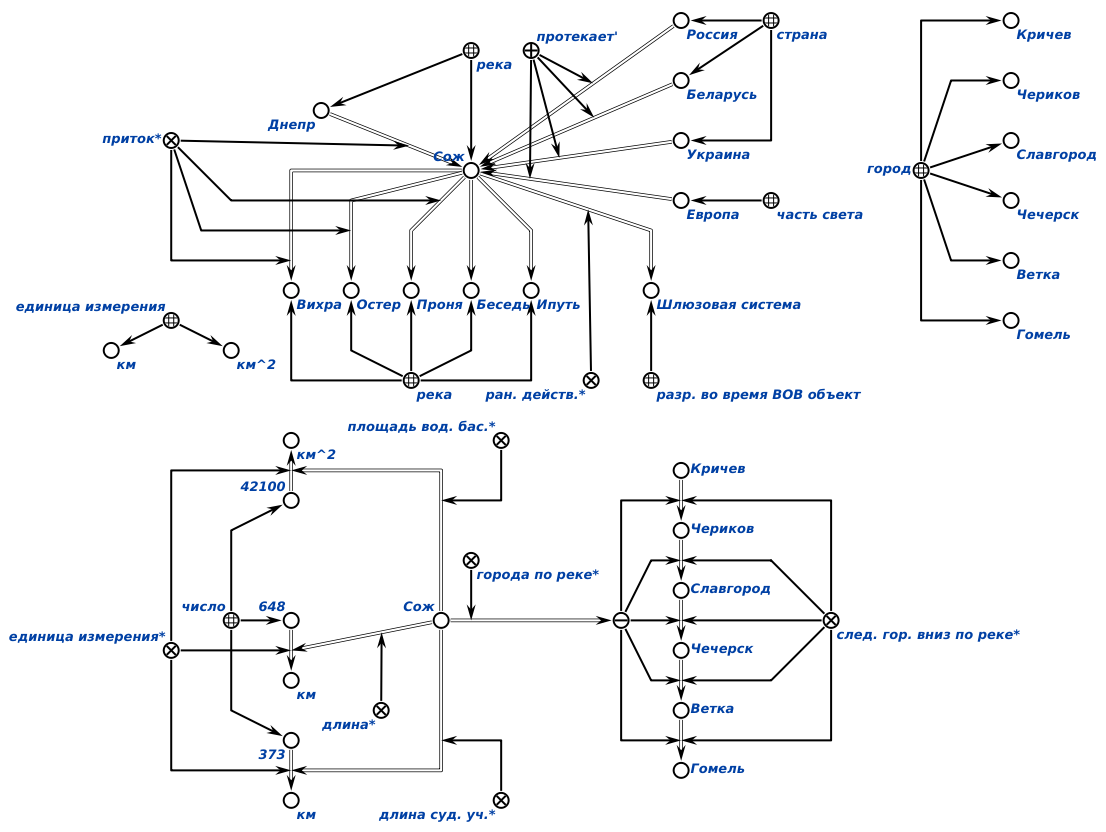
\includegraphics[scale=0.45]{images/work.png}
        }
    }
\scnaddlevel{-1}
\pagebreak
\scnhaselement{Пример формализации на SCg №2}
\scnaddlevel{1}
    \scntext{исходный текст}{ \(tg(3\alpha)=\frac{3tg\alpha-tg^{3}\alpha}{1-3tg^{2}\alpha}\) }
    \scnrelfrom{SCg}{
        \scnfileitem{\\
            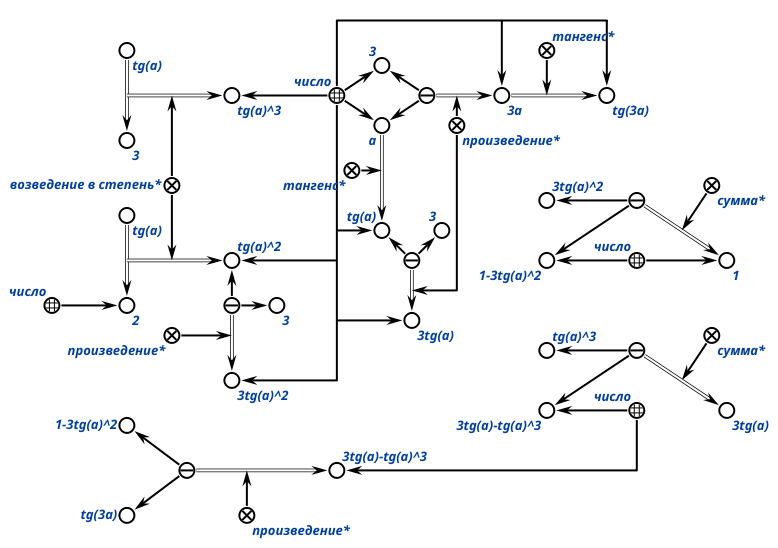
\includegraphics[scale=0.6]{images/work2.png}
        }
    }
\scnaddlevel{-1}
\end{small}
\end{SCn}